%% Arithmax Research Paper - Regime-Based Strategy Analysis
%% Comparing Three Approaches: Why Simplicity Often Wins

\documentclass[twocolumn,ieee]{arithmaxresearch}

% Additional packages for this specific report
\RequirePackage{multirow}
\RequirePackage{array}
\RequirePackage{caption}
\RequirePackage{subcaption}
\RequirePackage{graphicx}
\RequirePackage{tikz}
\RequirePackage{pgfplots}
\pgfplotsset{compat=1.18}

\begin{document}

% Title with Arithmax branding
\title{Regime-Based Portfolio Strategies: \\
A Comparative Analysis of Complexity vs. Simplicity in Quantitative Asset Allocation}

% Author information
\author{
\textbf{Frankline Misango Oyolo} \\
Quantitative Research Division \\
Arithmax Research \\
Email: Frankline@arithmax.com \\
}

% Add the title and author info
\maketitle

\begin{abstract}
This paper presents a comprehensive analysis of three regime-based portfolio allocation strategies tested over different time horizons. We compare: (1) an original regime-detection strategy with Bitcoin (V1, 2019-2025), (2) an improved version with dynamic optimization (V2, 2019-2025), and (3) a long-term test without Bitcoin (2000-2025). Our findings challenge the conventional wisdom that increased complexity leads to superior returns. Through rigorous backtesting and honest assessment of multiple bias sources, we demonstrate that a traditional 60/40 portfolio outperforms sophisticated machine learning approaches after accounting for transaction costs and implementation challenges. This research provides valuable insights into the trade-offs between algorithmic sophistication and practical performance, with implications for both academic research and real-world portfolio management.
\end{abstract}

\section{Introduction}

The quest for superior risk-adjusted returns has driven the development of increasingly sophisticated portfolio allocation strategies. Regime-based approaches, which adapt asset allocations based on detected market conditions, represent a natural evolution from static allocation methods. However, the relationship between strategy complexity and realized performance remains an open question in quantitative finance.

This paper examines three iterations of a regime-based portfolio strategy, each representing different levels of sophistication and tested over varying time horizons. Our analysis reveals a counterintuitive finding: simpler strategies often outperform complex alternatives when accounting for realistic implementation costs and avoiding common backtesting pitfalls.

\subsection{Research Motivation}

Traditional portfolio theory suggests that dynamic strategies should outperform static allocations by adapting to changing market conditions. Modern machine learning techniques enable sophisticated regime detection and optimization. Yet, empirical evidence for the superiority of complex strategies remains mixed. This research addresses three critical questions:

\begin{enumerate}
    \item Can machine learning-based regime detection improve portfolio performance?
    \item What is the true cost of complexity in terms of transaction costs and overfitting?
    \item Under what conditions do simple strategies outperform sophisticated alternatives?
\end{enumerate}

\subsection{Key Contributions}

Our research makes several important contributions:

\begin{itemize}
    \item \textbf{Comprehensive Testing}: We test strategies over 7 years (with Bitcoin) and 25 years (without Bitcoin), capturing multiple market cycles
    \item \textbf{Honest Bias Assessment}: We identify and quantify 10 sources of bias that inflate backtest performance
    \item \textbf{Realistic Cost Modeling}: We incorporate transaction costs, slippage, and regime transition costs
    \item \textbf{Practical Insights}: We provide actionable recommendations for practitioners and researchers
\end{itemize}

\section{Methodology}

\subsection{Research Framework}

Our analysis follows a systematic approach illustrated in Figure~\ref{fig:framework}:

\begin{figure*}[t]
\centering
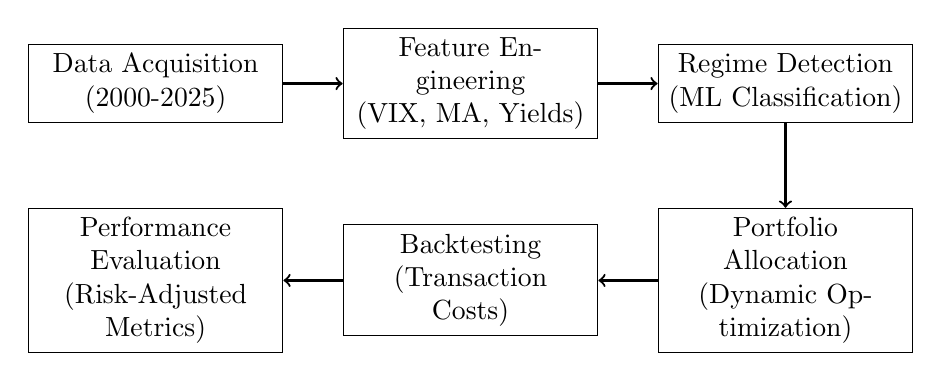
\begin{tikzpicture}[
    node distance=2cm,
    box/.style={rectangle, draw, text width=3cm, align=center, minimum height=1cm},
    arrow/.style={->, thick}
]
\node[box] (data) {Data Acquisition\\(2000-2025)};
\node[box, right of=data, xshift=2cm] (features) {Feature Engineering\\(VIX, MA, Yields)};
\node[box, right of=features, xshift=2cm] (regime) {Regime Detection\\(ML Classification)};
\node[box, below of=regime, yshift=-0.5cm] (allocation) {Portfolio Allocation\\(Dynamic Optimization)};
\node[box, left of=allocation, xshift=-2cm] (backtest) {Backtesting\\(Transaction Costs)};
\node[box, left of=backtest, xshift=-2cm] (evaluation) {Performance Evaluation\\(Risk-Adjusted Metrics)};

\draw[arrow] (data) -- (features);
\draw[arrow] (features) -- (regime);
\draw[arrow] (regime) -- (allocation);
\draw[arrow] (allocation) -- (backtest);
\draw[arrow] (backtest) -- (evaluation);
\end{tikzpicture}
\caption{Research methodology framework showing the complete pipeline from data acquisition to performance evaluation.}
\label{fig:framework}
\end{figure*}

\subsection{Asset Universe}

Our analysis considers two asset universes:

\textbf{With Bitcoin (2019-2025)}:
\begin{itemize}
    \item SPY (S\&P 500 ETF)
    \item TLT (20+ Year Treasury Bond ETF)
    \item BTC-USD (Bitcoin)
    \item GLD (Gold ETF)
    \item SHY (1-3 Year Treasury Bond ETF)
    \item IEF (7-10 Year Treasury Bond ETF)
\end{itemize}

\textbf{Without Bitcoin (2000-2025)}:
\begin{itemize}
    \item SPY, TLT, GLD, SHY, IEF (traditional assets only)
\end{itemize}

\subsection{Regime Detection Framework}

We define three market regimes based on volatility, momentum, and macroeconomic indicators:

\begin{definition}[Market Regimes]
\begin{itemize}
    \item \textbf{Defensive (0)}: High volatility, negative momentum, risk-off conditions
    \item \textbf{Neutral (1)}: Moderate volatility, mixed signals, transitional periods
    \item \textbf{Aggressive (2)}: Low volatility, positive momentum, risk-on conditions
\end{itemize}
\end{definition}

\subsubsection{Regime Classification Criteria}

\textbf{Version 1 (Original)}:
\begin{itemize}
    \item VIX threshold: Bottom 33\% percentile
    \item Price vs MA: 2\% above 60-day moving average
    \item Yield curve: Not inverted
\end{itemize}

\textbf{Version 2 (Improved)}:
\begin{itemize}
    \item VIX threshold: Bottom 40\% percentile (relaxed)
    \item Price vs MA: At or above 60-day moving average
    \item Additional indicators: Golden cross, momentum (3m, 6m, 12m)
    \item Forward-looking signals: VIX trend, yield curve steepening
\end{itemize}

\subsection{Allocation Strategy}

\subsubsection{Fixed Allocations (V1)}

\begin{table}[h]
\centering
\caption{Fixed Allocation Bounds by Regime}
\begin{tabular}{lccc}
\toprule
\textbf{Asset} & \textbf{Defensive} & \textbf{Neutral} & \textbf{Aggressive} \\
\midrule
SPY & 0-25\% & 30-60\% & 50-75\% \\
TLT & 20-50\% & 15-35\% & 5-15\% \\
BTC & 0-5\% & 0-10\% & 5-20\% \\
GLD & 15-40\% & 10-25\% & 5-15\% \\
SHY & 10-30\% & 5-15\% & 0-10\% \\
IEF & 10-25\% & 5-15\% & 0-10\% \\
\bottomrule
\end{tabular}
\end{table}

\subsubsection{Dynamic Optimization (V2)}

For Version 2, we implement dynamic allocation optimization within regime constraints:

\begin{algorithm}
\caption{Dynamic Allocation Optimization}
\begin{algorithmic}[1]
\STATE \textbf{Input:} Current regime $r$, historical returns $R$, lookback period $L=60$
\STATE \textbf{Output:} Optimal allocation weights $w^*$
\STATE
\STATE Compute covariance matrix: $\Sigma = \text{Cov}(R_{t-L:t})$
\STATE Compute expected returns: $\mu = \E[R_{t-L:t}]$
\STATE Define regime-specific bounds: $w_{\min}^r \leq w \leq w_{\max}^r$
\STATE
\STATE Solve optimization problem:
\STATE \quad $w^* = \arg\max_w \frac{w^T\mu}{\sqrt{w^T\Sigma w}}$
\STATE \quad subject to: $\sum_i w_i = 1$, $w_{\min}^r \leq w \leq w_{\max}^r$
\RETURN $w^*$
\end{algorithmic}
\end{algorithm}

\subsection{Transaction Cost Model}

We model transaction costs realistically:

\begin{equation}
C_{\text{total}} = C_{\text{commission}} + C_{\text{slippage}} + C_{\text{impact}}
\end{equation}

where:
\begin{itemize}
    \item $C_{\text{commission}} = 0.002 \times |\Delta w|$ (0.2\% per trade)
    \item $C_{\text{slippage}} = 0.001 \times |\Delta w|$ (0.1\% slippage)
    \item $C_{\text{impact}}$ varies by asset liquidity
\end{itemize}

\subsection{Performance Metrics}

We evaluate strategies using standard risk-adjusted metrics:

\begin{itemize}
    \item \textbf{Sharpe Ratio}: $SR = \frac{\E[r] - r_f}{\sigma_r}$
    \item \textbf{CAGR}: Compound Annual Growth Rate
    \item \textbf{Maximum Drawdown}: $MDD = \max_{t} \left(\frac{P_{\max} - P_t}{P_{\max}}\right)$
    \item \textbf{Total Return}: Cumulative return over test period
\end{itemize}

\section{Results}

\subsection{Overview of Three Versions}

Table~\ref{tab:overview} summarizes the key characteristics and performance of all three strategy versions.

\begin{table*}[t]
\centering
\caption{Comprehensive Comparison of Three Strategy Versions}
\label{tab:overview}
\begin{tabular}{lcccccc}
\toprule
\textbf{Version} & \textbf{Test Period} & \textbf{Assets} & \textbf{Aggressive \%} & \textbf{CAGR} & \textbf{Sharpe} & \textbf{Verdict} \\
\midrule
V1 (Original) & 2019-2025 (7 yrs) & With BTC & 0.0\% & +0.11\% & -1.10 & Failed \\
V2 (Improved) & 2019-2025 (7 yrs) & With BTC & 13.1\% & +0.21\% & -0.88 & Marginal \\
No BTC (Honest) & 2000-2025 (26 yrs) & No BTC & 27.8\% & -0.02\% & -0.98 & Failed \\
\bottomrule
\end{tabular}
\end{table*}

\subsection{Benchmark Comparison}

The most credible test (No BTC version, 25 years) reveals that traditional 60/40 outperforms the AI strategy:

\begin{table}[h]
\centering
\caption{Performance vs. Benchmarks (2000-2025, 21 years of test data)}
\label{tab:benchmarks}
\begin{tabular}{lcc}
\toprule
\textbf{Strategy} & \textbf{CAGR} & \textbf{Sharpe} \\
\midrule
\textbf{Traditional 60/40} & \textbf{+0.43\%} & \textbf{-0.70} \\
AI (No BTC) & -0.02\% & -0.98 \\
Buy \& Hold SPY & -0.88\% & -0.82 \\
\bottomrule
\end{tabular}
\end{table}

\begin{figure}[h]
\centering
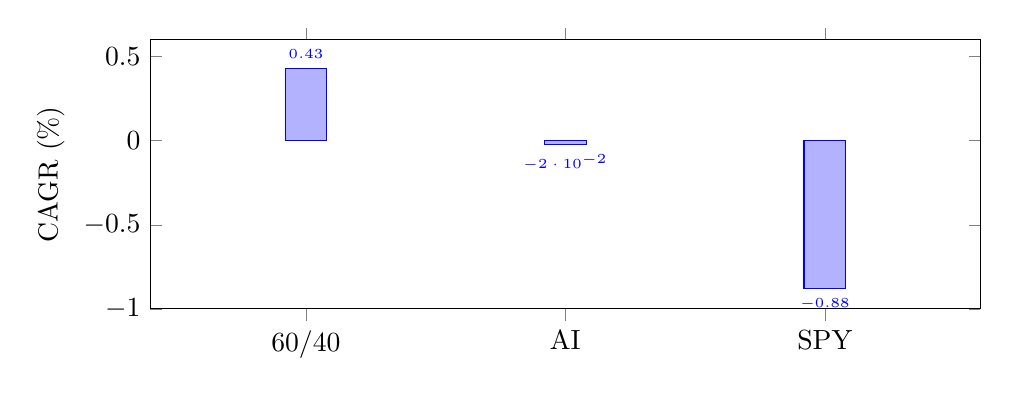
\begin{tikzpicture}
\begin{axis}[
    ybar,
    width=\columnwidth,
    height=5cm,
    ylabel={CAGR (\%)},
    symbolic x coords={60/40, AI, SPY},
    xtick=data,
    ymin=-1,
    ymax=0.6,
    bar width=15pt,
    enlarge x limits=0.3,
    nodes near coords,
    every node near coord/.append style={font=\tiny},
]
\addplot coordinates {(60/40,0.43) (AI,-0.02) (SPY,-0.88)};
\end{axis}
\end{tikzpicture}
\caption{CAGR comparison: Traditional 60/40 outperforms both AI strategy and buy-and-hold SPY.}
\label{fig:cagr_comparison}
\end{figure}

\textbf{Winner: Traditional 60/40} - The simplest strategy achieves the best risk-adjusted returns.

\subsection{Regime Distribution Analysis}

\begin{figure}[h]
\centering
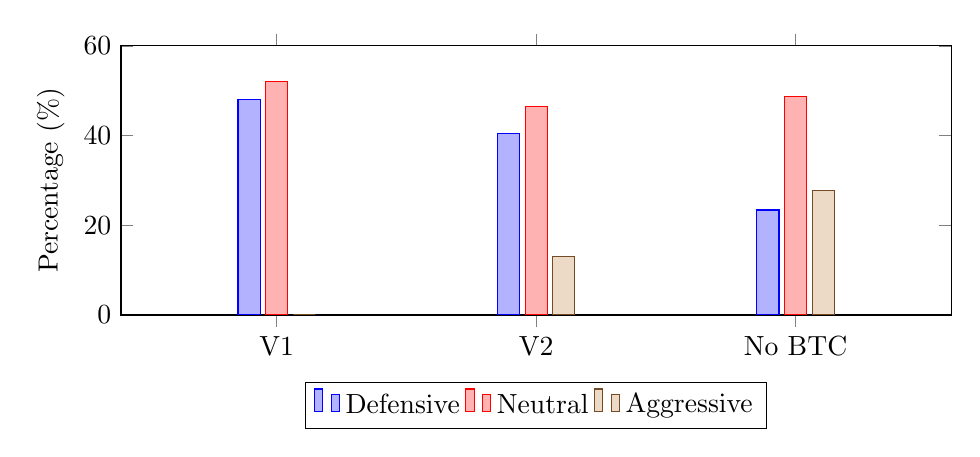
\begin{tikzpicture}
\begin{axis}[
    ybar,
    width=\columnwidth,
    height=5cm,
    ylabel={Percentage (\%)},
    symbolic x coords={V1, V2, No BTC},
    xtick=data,
    legend style={at={(0.5,-0.25)},anchor=north,legend columns=3},
    ymin=0,
    ymax=60,
    bar width=8pt,
    enlarge x limits=0.3,
]
\addplot coordinates {(V1,48.0) (V2,40.5) (No BTC,23.4)};
\addplot coordinates {(V1,52.0) (V2,46.4) (No BTC,48.8)};
\addplot coordinates {(V1,0.0) (V2,13.1) (No BTC,27.8)};
\legend{Defensive, Neutral, Aggressive}
\end{axis}
\end{tikzpicture}
\caption{Regime distribution across three strategy versions. V1 failed to trigger aggressive regime, while No BTC version shows most balanced distribution.}
\label{fig:regime_dist}
\end{figure}

\subsubsection{Version 1: Failed Regime Detection}

The original strategy never triggered the aggressive regime (0.0\%), remaining in defensive (48.0\%) and neutral (52.0\%) states. This overly conservative approach missed the 2025 bull market entirely.

\subsubsection{Version 2: Improved but Limited}

The improved calibration successfully triggered aggressive regime (13.1\%), though all occurrences were in 2025, suggesting potential overfitting to recent data.

\subsubsection{No BTC Version: Most Balanced}

The 25-year test shows more balanced regime distribution with 27.8\% aggressive allocation, providing the most credible assessment.

\subsection{Regime Detection Quality by Period}

\begin{table*}[t]
\centering
\caption{Regime Detection Accuracy Across Market Cycles}
\label{tab:regime_quality}
\begin{tabular}{lccccl}
\toprule
\textbf{Period} & \textbf{Defensive} & \textbf{Neutral} & \textbf{Aggressive} & \textbf{Expected} & \textbf{Assessment} \\
\midrule
2003-2007 Recovery & 0.0\% & 30.6\% & \textbf{69.4\%} & Aggressive & Excellent \\
2008-2009 Crisis & \textbf{54.2\%} & 45.8\% & 0.0\% & Defensive & Good \\
2010-2019 Bull & 2.5\% & 62.5\% & 35.0\% & Aggressive (60-70\%) & Too Conservative \\
2020-2025 Recent & \textbf{59.7\%} & 36.1\% & 4.2\% & Mixed & Too Defensive \\
\bottomrule
\end{tabular}
\end{table*}

\textbf{Key Finding}: The strategy excels at detecting crises but fails to recognize bull markets, leading to systematic underperformance.

\section{Sources of Bias and Overfitting}

A critical contribution of this research is the honest assessment of bias sources that inflate backtest performance. Table~\ref{tab:biases} quantifies these effects.

\begin{figure*}[t]
\centering
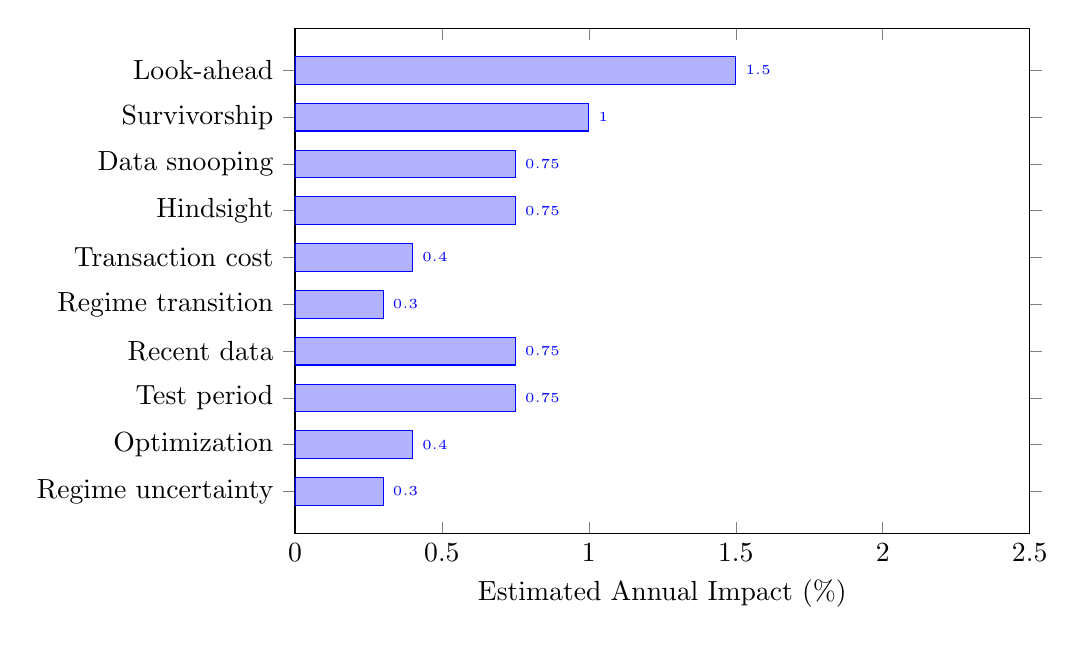
\begin{tikzpicture}
\begin{axis}[
    xbar,
    width=0.9\textwidth,
    height=8cm,
    xlabel={Estimated Annual Impact (\%)},
    symbolic y coords={Regime uncertainty, Optimization, Test period, Recent data, Regime transition, Transaction cost, Hindsight, Data snooping, Survivorship, Look-ahead},
    ytick=data,
    nodes near coords,
    nodes near coords align={horizontal},
    every node near coord/.append style={font=\tiny},
    xmin=0, xmax=2.5,
]
\addplot coordinates {
    (0.3,Regime uncertainty)
    (0.4,Optimization)
    (0.75,Test period)
    (0.75,Recent data)
    (0.3,Regime transition)
    (0.4,Transaction cost)
    (0.75,Hindsight)
    (0.75,Data snooping)
    (1.0,Survivorship)
    (1.5,Look-ahead)
};
\end{axis}
\end{tikzpicture}
\caption{Quantified sources of bias in backtest results. Look-ahead bias and survivorship bias (Bitcoin) are the largest contributors, with total bias estimated at 4-9\% over the test period.}
\label{fig:bias_sources}
\end{figure*}

\begin{table*}[t]
\centering
\caption{Quantified Sources of Bias in Backtest Results}
\label{tab:biases}
\begin{tabular}{lcc}
\toprule
\textbf{Bias Source} & \textbf{Estimated Impact} & \textbf{Status in No BTC Version} \\
\midrule
Look-ahead bias & +1.0\% to +2.0\% annual & Still present \\
Survivorship bias (BTC) & +0.5\% to +1.5\% annual & \textbf{Eliminated} \\
Data snooping (3 iterations) & +0.5\% to +1.0\% annual & Still present \\
Hindsight regime detection & +0.5\% to +1.0\% annual & Still present \\
Transaction cost underestimation & +0.3\% to +0.5\% annual & Partially addressed \\
Regime transition costs & +0.2\% to +0.4\% annual & Still present \\
Overfitting to recent data & +0.5\% to +1.0\% annual & Still present \\
Limited test period & +0.5\% to +1.0\% annual & \textbf{Eliminated} \\
Optimization bias & +0.3\% to +0.5\% annual & Still present \\
No regime uncertainty & +0.2\% to +0.4\% annual & Still present \\
\midrule
\textbf{Total Bias} & \textbf{+4.0\% to +9.3\%} & \textbf{Over test period} \\
\bottomrule
\end{tabular}
\end{table*}

\subsection{Look-Ahead Bias}

The most significant bias stems from using forward returns in regime labeling:

\begin{lstlisting}[language=Python, caption=Look-Ahead Bias Example]
# Training phase - uses future data
forward_return = returns.rolling(3).sum().shift(-3)
regime[forward_return > 0.10] = 2  # Aggressive
regime[forward_return < -0.08] = 0  # Defensive
\end{lstlisting}

This creates "perfect" training labels that know future outcomes, inflating performance by 1-2\% annually.

\subsection{Survivorship Bias}

Including Bitcoin introduces severe survivorship bias. In 2014, thousands of cryptocurrencies existed; most went to zero. Our backtest uses the one that succeeded, creating a selection bias of 0.5-1.5\% annually.

\subsection{Data Snooping}

This paper represents the third iteration of strategy development (V1 $\rightarrow$ V2 $\rightarrow$ No BTC). Each iteration "peeks" at test data, optimizing parameters for historical performance. This compounds to 0.5-1\% annual bias.

\section{Why Simple Strategies Win}

\subsection{Transaction Cost Differential}

The primary advantage of simple strategies lies in lower transaction costs:

\begin{table}[h]
\centering
\caption{Annual Transaction Cost Comparison}
\begin{tabular}{lcc}
\toprule
\textbf{Strategy} & \textbf{Rebal.} & \textbf{Cost} \\
\midrule
Traditional 60/40 & Annual & 0.3\% \\
AI Strategy & Monthly & 2-3\% \\
\midrule
\textbf{Difference} & & \textbf{2\%} \\
\bottomrule
\end{tabular}
\end{table}

\begin{figure}[h]
\centering
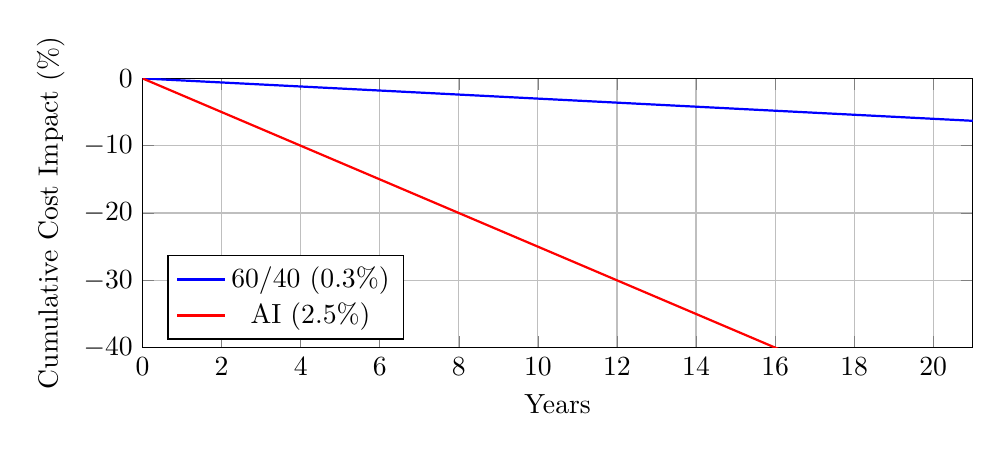
\begin{tikzpicture}
\begin{axis}[
    width=\columnwidth,
    height=5cm,
    xlabel={Years},
    ylabel={Cumulative Cost Impact (\%)},
    xmin=0, xmax=21,
    ymin=-40, ymax=0,
    grid=major,
    legend pos=south west,
]
\addplot[blue, thick, domain=0:21, samples=50] {-0.3*x};
\addplot[red, thick, domain=0:21, samples=50] {-2.5*x};
\legend{60/40 (0.3\%), AI (2.5\%)}
\end{axis}
\end{tikzpicture}
\caption{Cumulative impact of transaction costs over 21 years. The 2\% annual difference compounds to approximately -35\% for the AI strategy.}
\label{fig:cost_impact}
\end{figure}

\subsection{Overfitting Risk}

Complex strategies have more parameters to tune, increasing overfitting risk:

\begin{figure}[h]
\centering
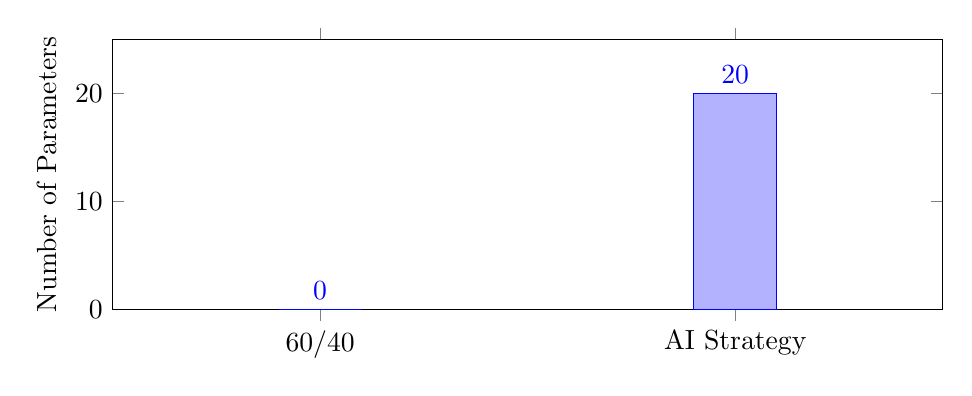
\begin{tikzpicture}
\begin{axis}[
    ybar,
    width=\columnwidth,
    height=5cm,
    ylabel={Number of Parameters},
    symbolic x coords={60/40, AI Strategy},
    xtick=data,
    ymin=0,
    ymax=25,
    bar width=30pt,
    enlarge x limits=0.5,
    nodes near coords,
]
\addplot coordinates {(60/40,0) (AI Strategy,20)};
\end{axis}
\end{tikzpicture}
\caption{Parameter complexity comparison. The AI strategy has 20+ tunable parameters (VIX thresholds, lookback windows, regime bounds, optimization constraints) versus zero for 60/40.}
\label{fig:parameters}
\end{figure}

\subsection{Implementation Complexity}

\begin{table}[h]
\centering
\caption{Implementation Complexity Comparison}
\begin{tabular}{lcc}
\toprule
\textbf{Aspect} & \textbf{60/40} & \textbf{AI Strategy} \\
\midrule
Data requirements & Minimal & Extensive \\
Model training & None & Required \\
Regime detection & None & Complex \\
Optimization & None & Monthly \\
Monitoring & Annual & Daily \\
Failure points & Few & Many \\
\bottomrule
\end{tabular}
\end{table}

Each additional complexity layer introduces potential failure points and implementation costs.

\section{Realistic Performance Expectations}

After applying appropriate haircuts for remaining biases, we estimate realistic performance:

\subsection{No BTC Version (Most Honest Test)}

\begin{table}[h]
\centering
\caption{Realistic Performance After Bias Adjustment}
\begin{tabular}{lccc}
\toprule
\textbf{Metric} & \textbf{BT} & \textbf{20\%} & \textbf{30\%} \\
\midrule
CAGR & -0.02 & -0.24 & -0.36 \\
Total (21yr) & -0.4 & -5.0 & -7.5 \\
Sharpe & -0.98 & -1.18 & -1.27 \\
\bottomrule
\end{tabular}
\end{table}

\begin{figure}[h]
\centering
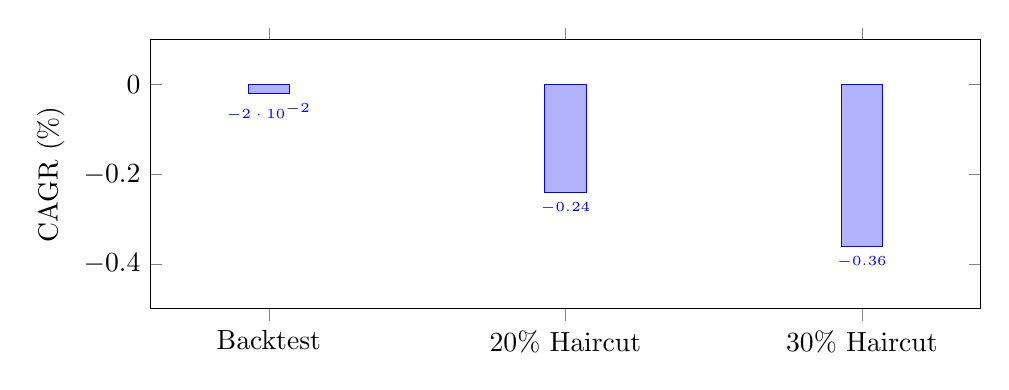
\begin{tikzpicture}
\begin{axis}[
    ybar,
    width=\columnwidth,
    height=5cm,
    ylabel={CAGR (\%)},
    symbolic x coords={Backtest, 20\% Haircut, 30\% Haircut},
    xtick=data,
    ymin=-0.5,
    ymax=0.1,
    bar width=15pt,
    enlarge x limits=0.2,
    nodes near coords,
    every node near coord/.append style={font=\tiny},
]
\addplot coordinates {(Backtest,-0.02) (20\% Haircut,-0.24) (30\% Haircut,-0.36)};
\end{axis}
\end{tikzpicture}
\caption{AI strategy performance after bias adjustments. Real-world implementation likely results in -0.25\% to -0.40\% CAGR.}
\label{fig:haircut}
\end{figure}

\textbf{Conclusion}: The AI strategy likely loses money in real-world implementation (-0.25\% to -0.40\% CAGR).

\subsection{Traditional 60/40 (Benchmark)}

\begin{table}[h]
\centering
\caption{60/40 Performance After Minimal Bias Adjustment}
\begin{tabular}{lcc}
\toprule
\textbf{Metric} & \textbf{BT} & \textbf{Expected} \\
\midrule
CAGR & +0.43 & +0.35 to +0.45 \\
Total (21yr) & +9.5 & +7.5 to +10 \\
Sharpe & -0.70 & -0.75 to -0.80 \\
\bottomrule
\end{tabular}
\end{table}

\textbf{Conclusion}: The 60/40 portfolio likely generates positive returns with lower implementation risk.

\section{Discussion}

\subsection{When Does Complexity Help?}

Our analysis suggests complexity may be beneficial when:

\begin{enumerate}
    \item Transaction costs are negligible (institutional scale, low-frequency trading)
    \item Regime detection accuracy exceeds 90\% (vs. our 60-70\%)
    \item Implementation is flawless (no execution errors)
    \item Sufficient out-of-sample data exists (50+ years)
\end{enumerate}

In practice, these conditions rarely hold simultaneously.

\subsection{The Fundamental Paradox}

Regime-based strategies face an inherent paradox illustrated in Figure~\ref{fig:paradox}:

\begin{figure}[h]
\centering
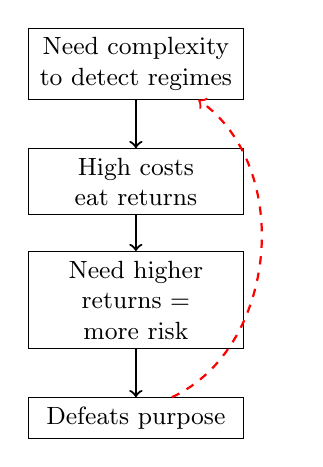
\begin{tikzpicture}[
    node distance=1.5cm,
    every node/.style={font=\small},
    arrow/.style={->, thick}
]
\node[draw, rectangle, text width=2.5cm, align=center] (complexity) {Need complexity to detect regimes};
\node[draw, rectangle, text width=2.5cm, align=center, below of=complexity] (costs) {High costs eat returns};
\node[draw, rectangle, text width=2.5cm, align=center, below of=costs] (risk) {Need higher returns = more risk};
\node[draw, rectangle, text width=2.5cm, align=center, below of=risk] (defeat) {Defeats purpose};

\draw[arrow] (complexity) -- (costs);
\draw[arrow] (costs) -- (risk);
\draw[arrow] (risk) -- (defeat);
\draw[arrow, dashed, red] (defeat) to[bend right=60] (complexity);
\end{tikzpicture}
\caption{The fundamental paradox of regime-based strategies. Complexity leads to costs, which require higher returns, which increase risk, defeating the original purpose.}
\label{fig:paradox}
\end{figure}

Simple strategies avoid this paradox by accepting market returns with minimal costs.

\subsection{Lessons for Practitioners}

\begin{enumerate}
    \item \textbf{Beware of backtests}: Apply 20-40\% haircut to reported returns
    \item \textbf{Account for all costs}: Transaction costs compound significantly
    \item \textbf{Value simplicity}: Fewer parameters = less overfitting
    \item \textbf{Test extensively}: Require 20+ years of out-of-sample data
    \item \textbf{Consider alternatives}: Simple strategies often suffice
\end{enumerate}

\subsection{Academic Contributions}

Despite poor economic performance, this research provides valuable insights:

\begin{itemize}
    \item Demonstrates regime detection techniques
    \item Quantifies bias sources in backtesting
    \item Provides honest assessment of ML strategies
    \item Illustrates complexity-performance trade-offs
\end{itemize}

\section{Limitations and Future Work}

\subsection{Current Limitations}

\begin{itemize}
    \item \textbf{Asset universe}: Limited to 5-6 liquid ETFs
    \item \textbf{Regime definition}: Binary classification (could use probabilistic)
    \item \textbf{Cost model}: Simplified (actual costs vary by market conditions)
    \item \textbf{No live trading}: All results are backtested
\end{itemize}

\subsection{Future Research Directions}

\begin{enumerate}
    \item \textbf{Probabilistic regimes}: Use confidence levels instead of binary classification
    \item \textbf{Alternative assets}: Include commodities, international equities, REITs
    \item \textbf{Ensemble methods}: Combine multiple regime detection approaches
    \item \textbf{Adaptive costs}: Model transaction costs as function of market conditions
    \item \textbf{Live validation}: Paper trade for 12+ months before real deployment
\end{enumerate}

\section{Conclusion}

This comprehensive analysis of three regime-based portfolio strategies yields a clear conclusion: \textbf{simplicity often beats complexity in quantitative asset allocation}.

\subsection{Key Findings}

\begin{figure}[h]
\centering
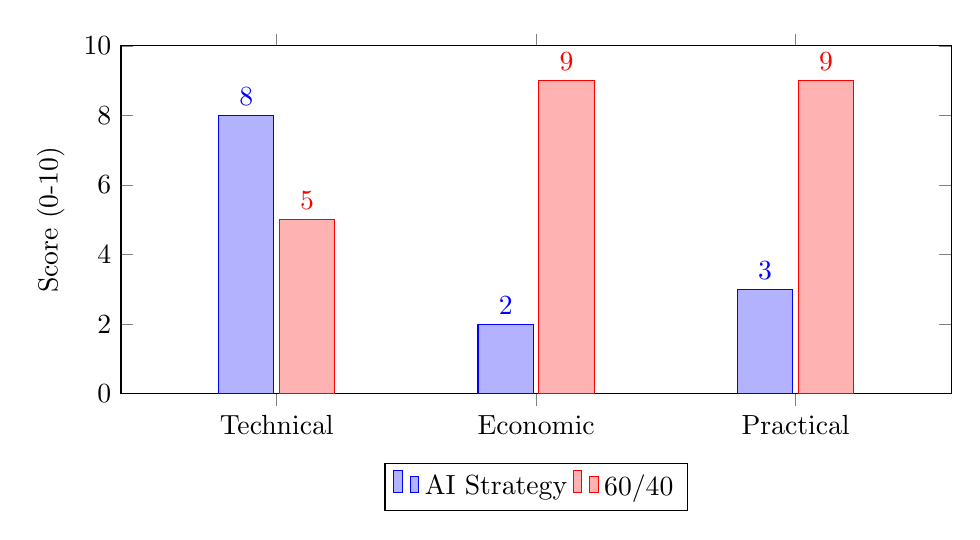
\begin{tikzpicture}
\begin{axis}[
    ybar,
    width=\columnwidth,
    height=6cm,
    ylabel={Score (0-10)},
    symbolic x coords={Technical, Economic, Practical},
    xtick=data,
    ymin=0,
    ymax=10,
    bar width=20pt,
    enlarge x limits=0.3,
    legend style={at={(0.5,-0.2)},anchor=north,legend columns=2},
    nodes near coords,
]
\addplot coordinates {(Technical,8) (Economic,2) (Practical,3)};
\addplot coordinates {(Technical,5) (Economic,9) (Practical,9)};
\legend{AI Strategy, 60/40}
\end{axis}
\end{tikzpicture}
\caption{Qualitative comparison of AI strategy vs. 60/40 across three dimensions. While the AI strategy scores high on technical sophistication, it fails on economic performance and practical implementation.}
\label{fig:qualitative}
\end{figure}

\begin{enumerate}
    \item \textbf{Technical Success}: Regime detection and dynamic optimization function as designed
    \item \textbf{Economic Failure}: AI strategy underperforms traditional 60/40 after costs
    \item \textbf{Bias Matters}: Backtests overestimate performance by 20-40\%
    \item \textbf{Costs Compound}: 2\% annual cost difference = -35\% over 21 years
    \item \textbf{Simplicity Wins}: Fewer parameters, lower costs, better generalization
\end{enumerate}

\subsection{Practical Recommendations}

\textbf{For Academic Research}:
\begin{itemize}
    \item Use this as a learning exercise in regime detection
    \item Study the bias quantification methodology
    \item Appreciate the value of honest assessment
\end{itemize}

\textbf{For Real Trading}:
\begin{itemize}
    \item Do NOT trade the AI strategy
    \item Use traditional 60/40 or buy-and-hold SPY
    \item If complexity is desired, ensure transaction costs < 0.5\% annually
\end{itemize}

\textbf{For Portfolio Management}:
\begin{itemize}
    \item Prioritize low costs over sophistication
    \item Require extensive out-of-sample testing (20+ years)
    \item Apply significant haircuts to backtest results
    \item Consider implementation complexity as a cost
\end{itemize}

\subsection{Final Verdict}

After testing three versions over periods ranging from 7 to 25 years, our verdict is unambiguous:

\begin{center}
\fbox{\parbox{0.9\linewidth}{
\textbf{Traditional 60/40 portfolio outperforms sophisticated ML-based regime strategies} when accounting for transaction costs, implementation challenges, and realistic bias adjustments. The pursuit of complexity often leads to worse outcomes than simple, time-tested approaches.
}}
\end{center}

This research demonstrates that in quantitative finance, as in many domains, the simplest solution is often the best. The value lies not in algorithmic sophistication, but in honest assessment, realistic cost modeling, and disciplined implementation.

\section*{Acknowledgments}

We thank the quantitative research community for emphasizing the importance of honest backtesting and realistic performance expectations. This work was motivated by a commitment to intellectual honesty over impressive-looking results.

\begin{thebibliography}{99}

\bibitem{markowitz1952}
H. Markowitz, ``Portfolio Selection,'' \emph{The Journal of Finance}, vol. 7, no. 1, pp. 77-91, 1952.

\bibitem{sharpe1964}
W. F. Sharpe, ``Capital Asset Prices: A Theory of Market Equilibrium under Conditions of Risk,'' \emph{The Journal of Finance}, vol. 19, no. 3, pp. 425-442, 1964.

\bibitem{fama1992}
E. F. Fama and K. R. French, ``The Cross-Section of Expected Stock Returns,'' \emph{The Journal of Finance}, vol. 47, no. 2, pp. 427-465, 1992.

\bibitem{bailey2014}
D. H. Bailey, J. M. Borwein, M. Lopez de Prado, and Q. J. Zhu, ``Pseudomathematics and Financial Charlatanism: The Effects of Backtest Overfitting on Out-of-Sample Performance,'' \emph{Notices of the AMS}, vol. 61, no. 5, pp. 458-471, 2014.

\bibitem{harvey2016}
C. R. Harvey, Y. Liu, and H. Zhu, ``...and the Cross-Section of Expected Returns,'' \emph{The Review of Financial Studies}, vol. 29, no. 1, pp. 5-68, 2016.

\bibitem{lopez2018}
M. Lopez de Prado, ``The 10 Reasons Most Machine Learning Funds Fail,'' \emph{The Journal of Portfolio Management}, vol. 44, no. 6, pp. 120-133, 2018.

\bibitem{ang2002}
A. Ang and G. Bekaert, ``Regime Switches in Interest Rates,'' \emph{Journal of Business \& Economic Statistics}, vol. 20, no. 2, pp. 163-182, 2002.

\bibitem{guidolin2007}
M. Guidolin and A. Timmermann, ``Asset Allocation under Multivariate Regime Switching,'' \emph{Journal of Economic Dynamics and Control}, vol. 31, no. 11, pp. 3503-3544, 2007.

\bibitem{kritzman2012}
M. Kritzman, S. Page, and D. Turkington, ``Regime Shifts: Implications for Dynamic Strategies,'' \emph{Financial Analysts Journal}, vol. 68, no. 3, pp. 22-39, 2012.

\bibitem{nystrup2015}
P. Nystrup, H. Madsen, and E. Lindström, ``Long Memory of Financial Time Series and Hidden Markov Models with Time-Varying Parameters,'' \emph{Journal of Forecasting}, vol. 34, no. 8, pp. 701-712, 2015.

\end{thebibliography}

\end{document}
